\section{(W) Remaining "Well Clear"}\label{sec:WellClear}
    \begin{itemize}
        \item Well clear definition/Near miss definition
        \item Well clear zones (Crash margin (near miss), warning margin, alert margin)
    \end{itemize}
    \begin{figure}[H]
        \centering
        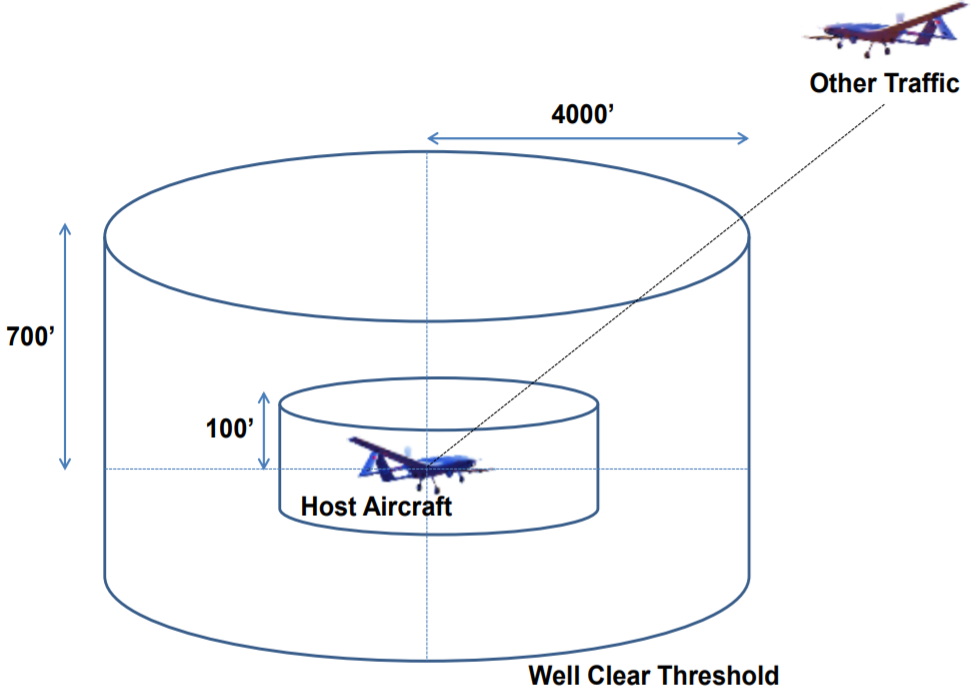
\includegraphics[width=0.6\textwidth]{\FIGDIR/02_05_WellClearTreshold}
        \caption{Well Clear Threshold \cite{valavanis2015uav,united1983pilots}.}
        \label{fig:WellClearTreshold}
    \end{figure}


\subsection{(W) Air Traffic Control(ATC)}\label{sec:AirTrafficControl}
    \begin{itemize}
        \item Keeping Aircraft$\leftrightarrow$ UTM $\leftrightarrow$ Aircraft well clear
        \item ATC situations - Climb/Descent/Leveled flight (presentation), put emphasis on horizontal/vertical separation
        \item warning/notice/resolution notation and definitions
        \item standard ATM functionality
        \item Standard procedures convergence/divergence
        \item Standard procedures for maneuver restrictions
    \end{itemize}
    
    Real-time \emph{Airspace Management} approach have been presented in \cite{gardi2014real}. Following \emph{Dynamic Airspace Management} \cite{gerdes2016dynamic}.
    \begin{figure}[H]
        \centering
        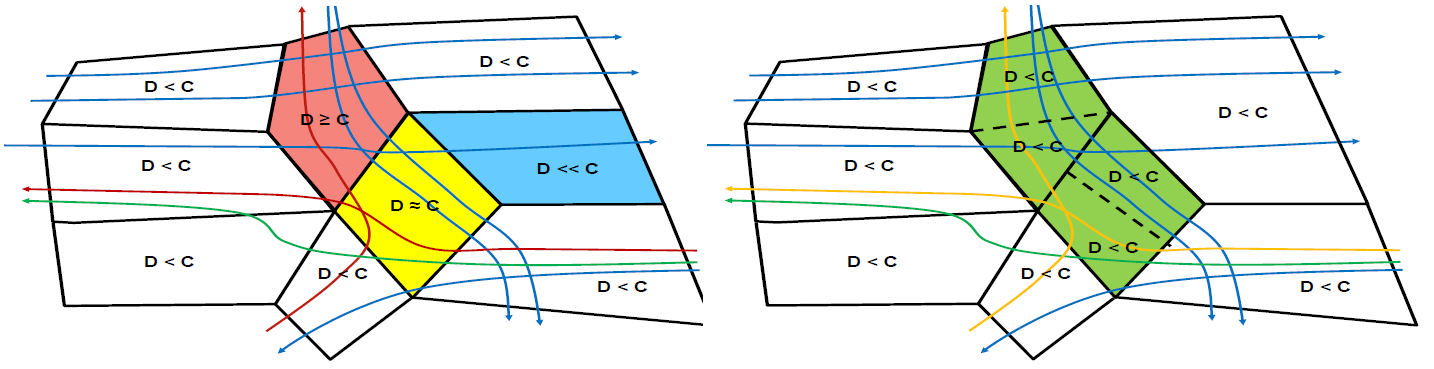
\includegraphics[width=1\textwidth]{\FIGDIR/02_02_DAM_Example}
        \caption{Example of DAM flight rerouting to homogenize traffic density \cite{gerdes2016dynamic}.}
        \label{fig:DAMExample}
    \end{figure}


\subsection{(W) Traffic Collision Avoidance System (TCAS)}\label{sec:TCAS}
\begin{itemize}
    \item Keeping Aircraft $\leftrightarrow$ Aircraft well clear,
    \item Traffic advisories and alerts messaging,
    \item Basic principle dissemination,
\end{itemize}

\subsection{(W) Airborne Collision Avoidance System X  (ACAS-X)}\label{sec:ACASX}
\emph{ACAS-$X_U$} concept have been implemented as \emph{Deep Neural Network Solver} in \cite{katz2017reluplex}
\begin{itemize}
    \item ACAS principples
    \item AXAS XA addition TCAS
\end{itemize}

